\begin{tcolorbox}[posterbox]
\SectionTitle{ERP Results: MMN and N1 Scaling}
\SmallText
Representative no-topo overlays from key analyses.

\vspace{0.2em}
\begin{center}
\begin{tabular}{cc}
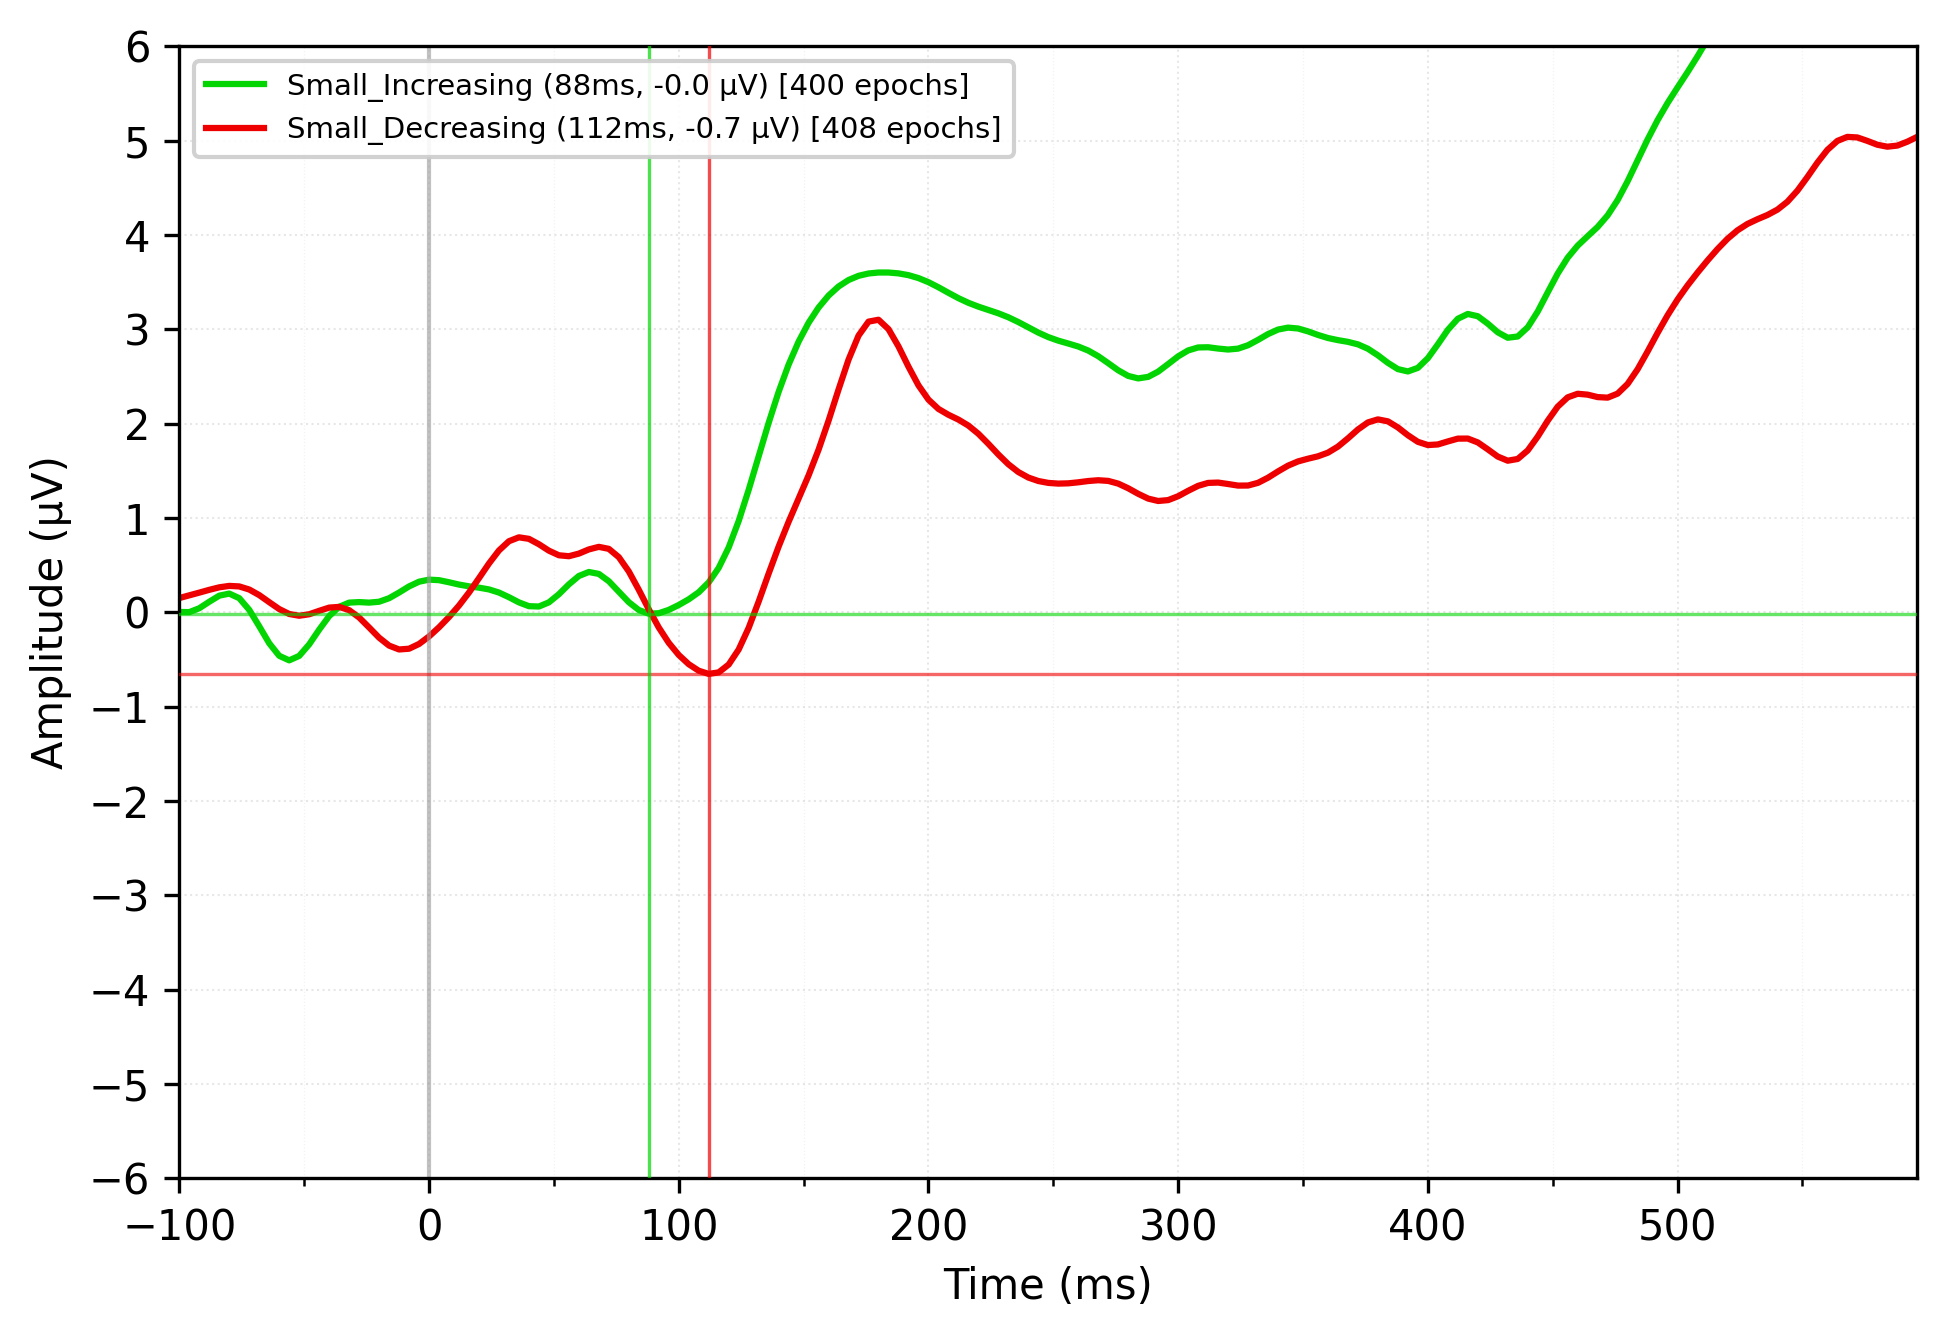
\includegraphics[width=0.43\linewidth]{../docs/assets/plots/small_increasing_vs_decreasing_ACC1/small_increasing_vs_decreasing_ACC1-Fz-no_topo.png} &
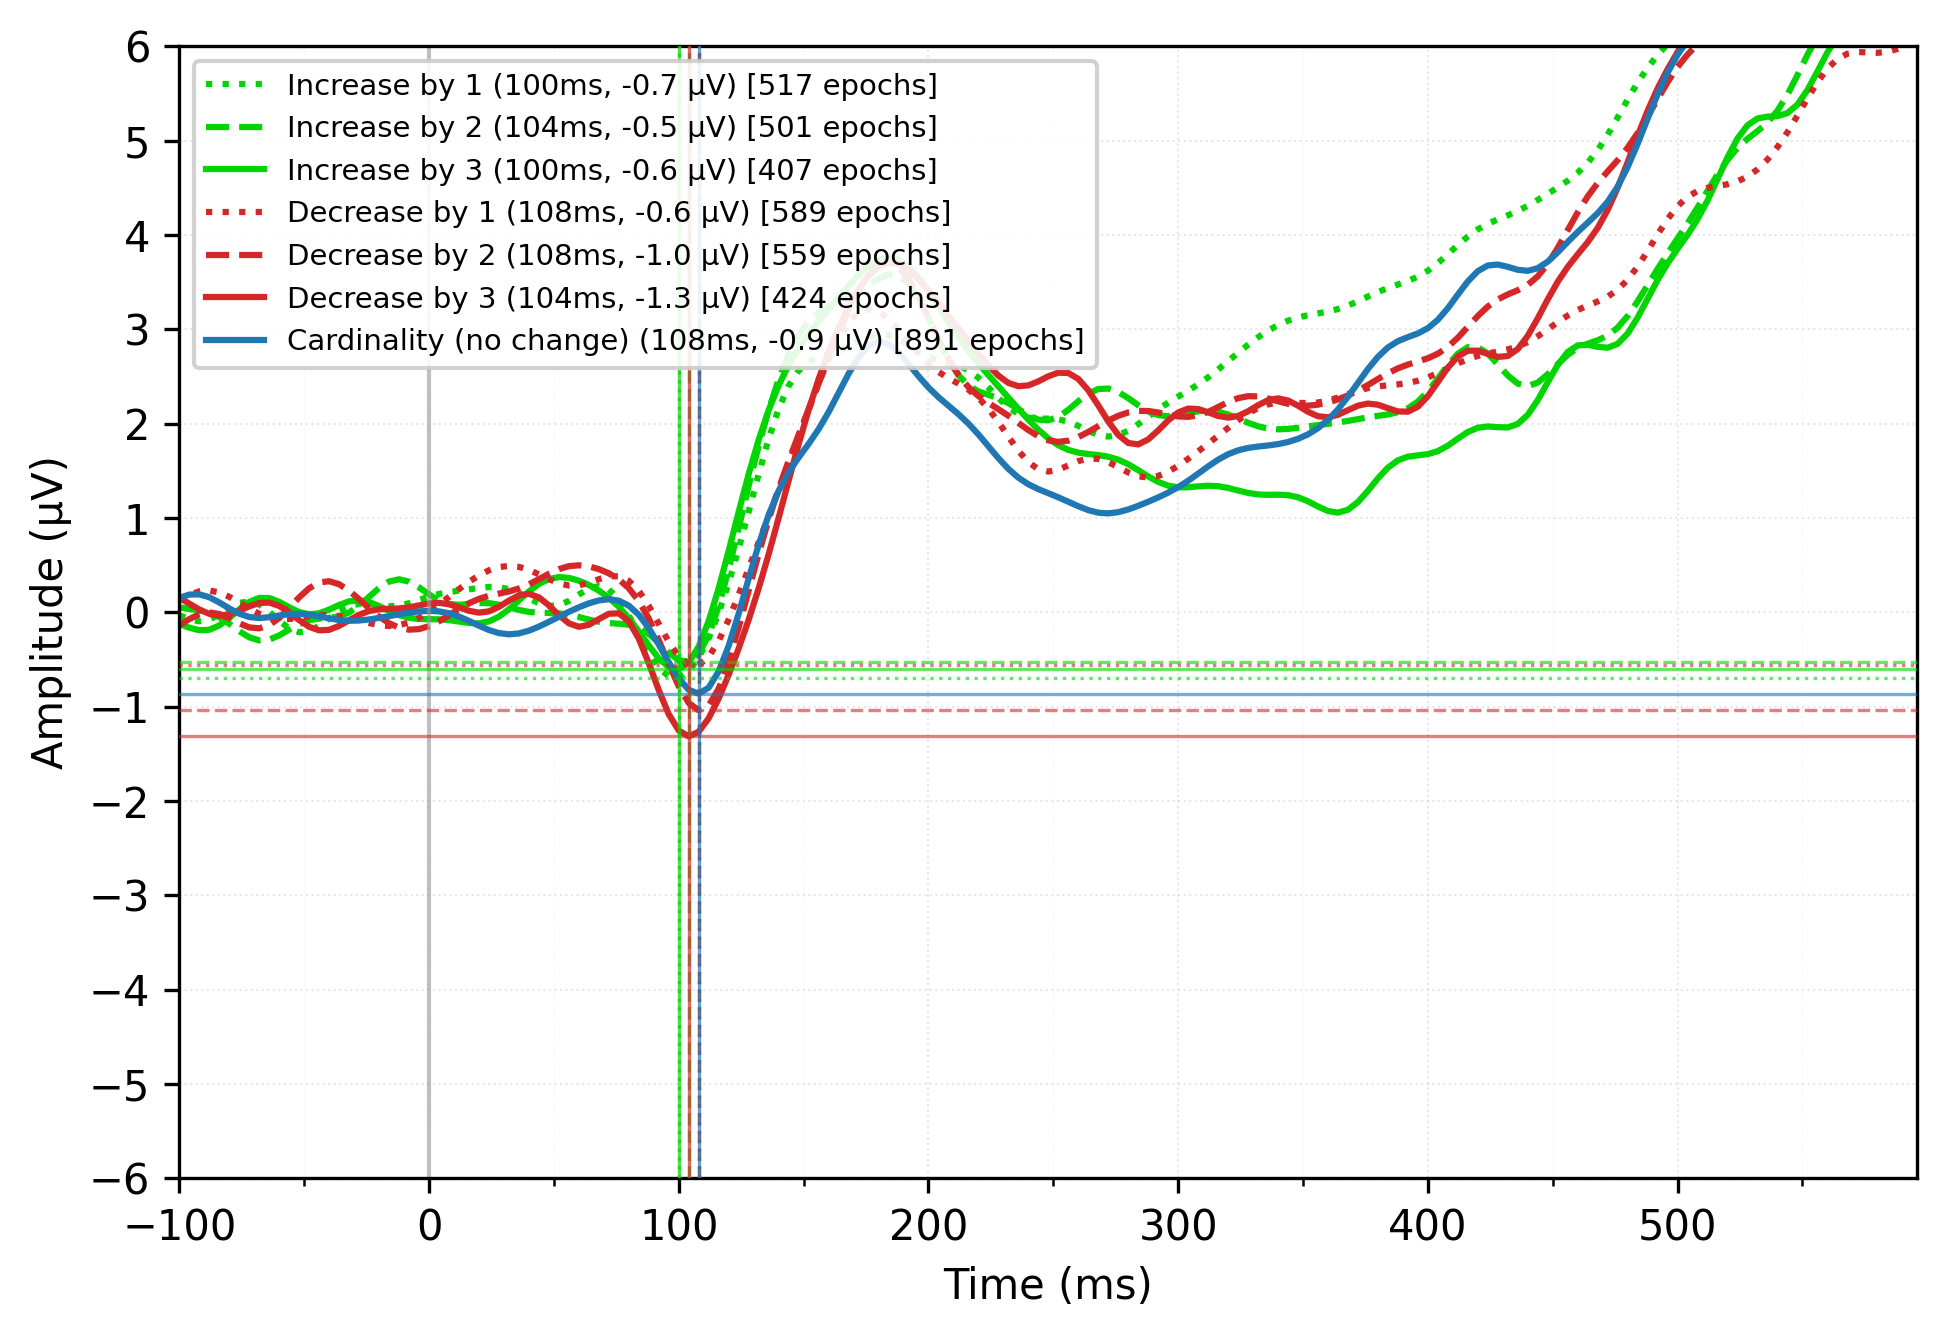
\includegraphics[width=0.43\linewidth]{../docs/assets/plots/increase_decrease_123_ACC1/increase_decrease_123_ACC1-Fz-no_topo.png} \\
[0.12em]
{\fontsize{14}{17}\selectfont Direction contrast at Fz} &
{\fontsize{14}{17}\selectfont Distance contrast at Fz} \\
[0.25em]
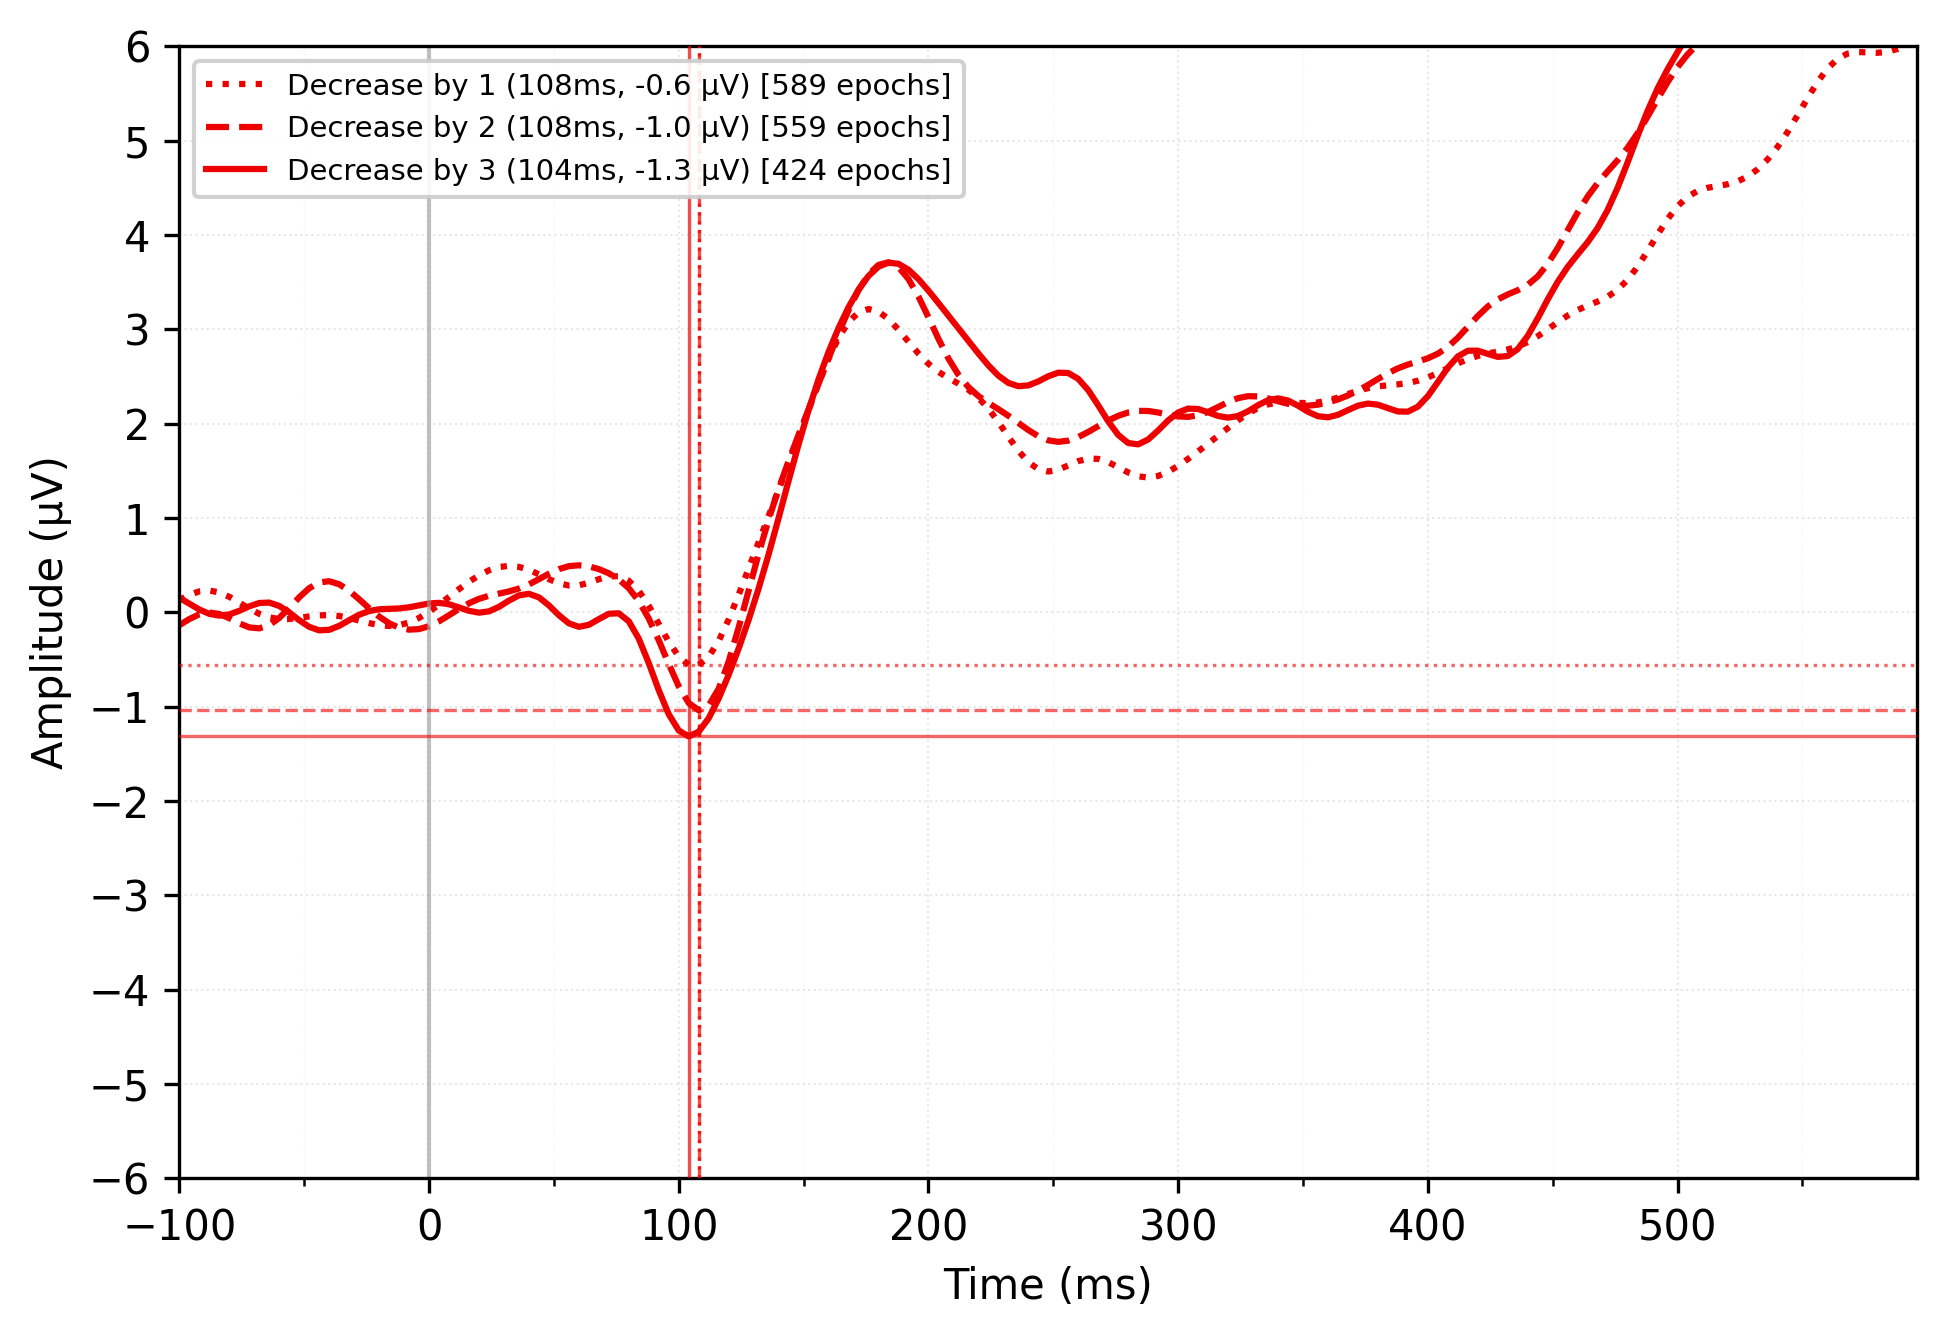
\includegraphics[width=0.43\linewidth]{../docs/assets/plots/decrease_by_123_ACC1/decrease_by_123_ACC1-Fz-no_topo.png} &
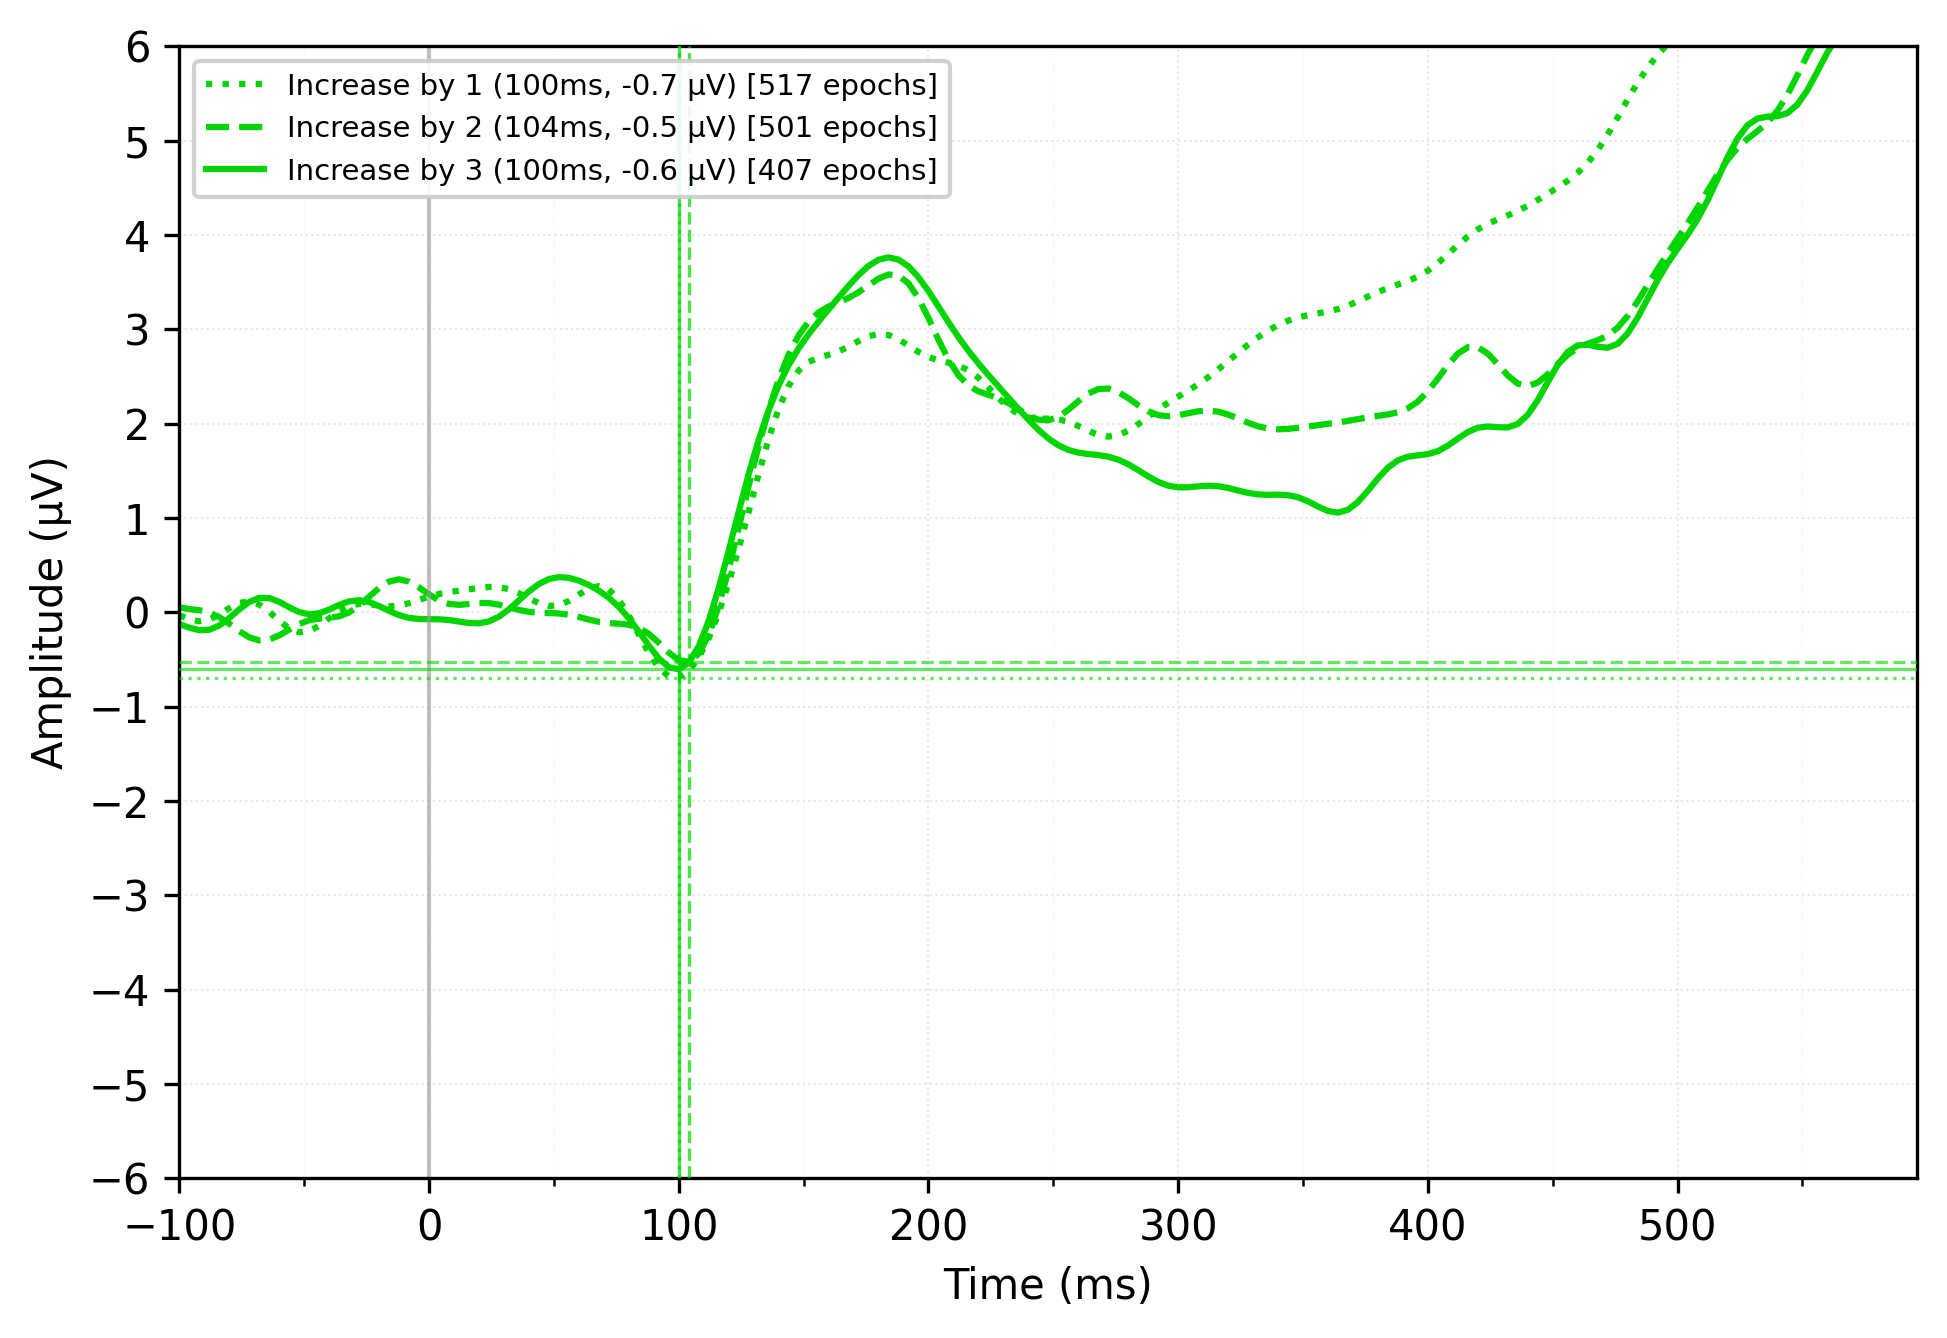
\includegraphics[width=0.43\linewidth]{../docs/assets/plots/increase_by_123_ACC1/increase_by_123_ACC1-Fz-no_topo.png} \\
[0.12em]
{\fontsize{14}{17}\selectfont Decreasing-only (Diff 1-3)} &
{\fontsize{14}{17}\selectfont Increasing-only (Diff 1-3)} \\
[0.25em]
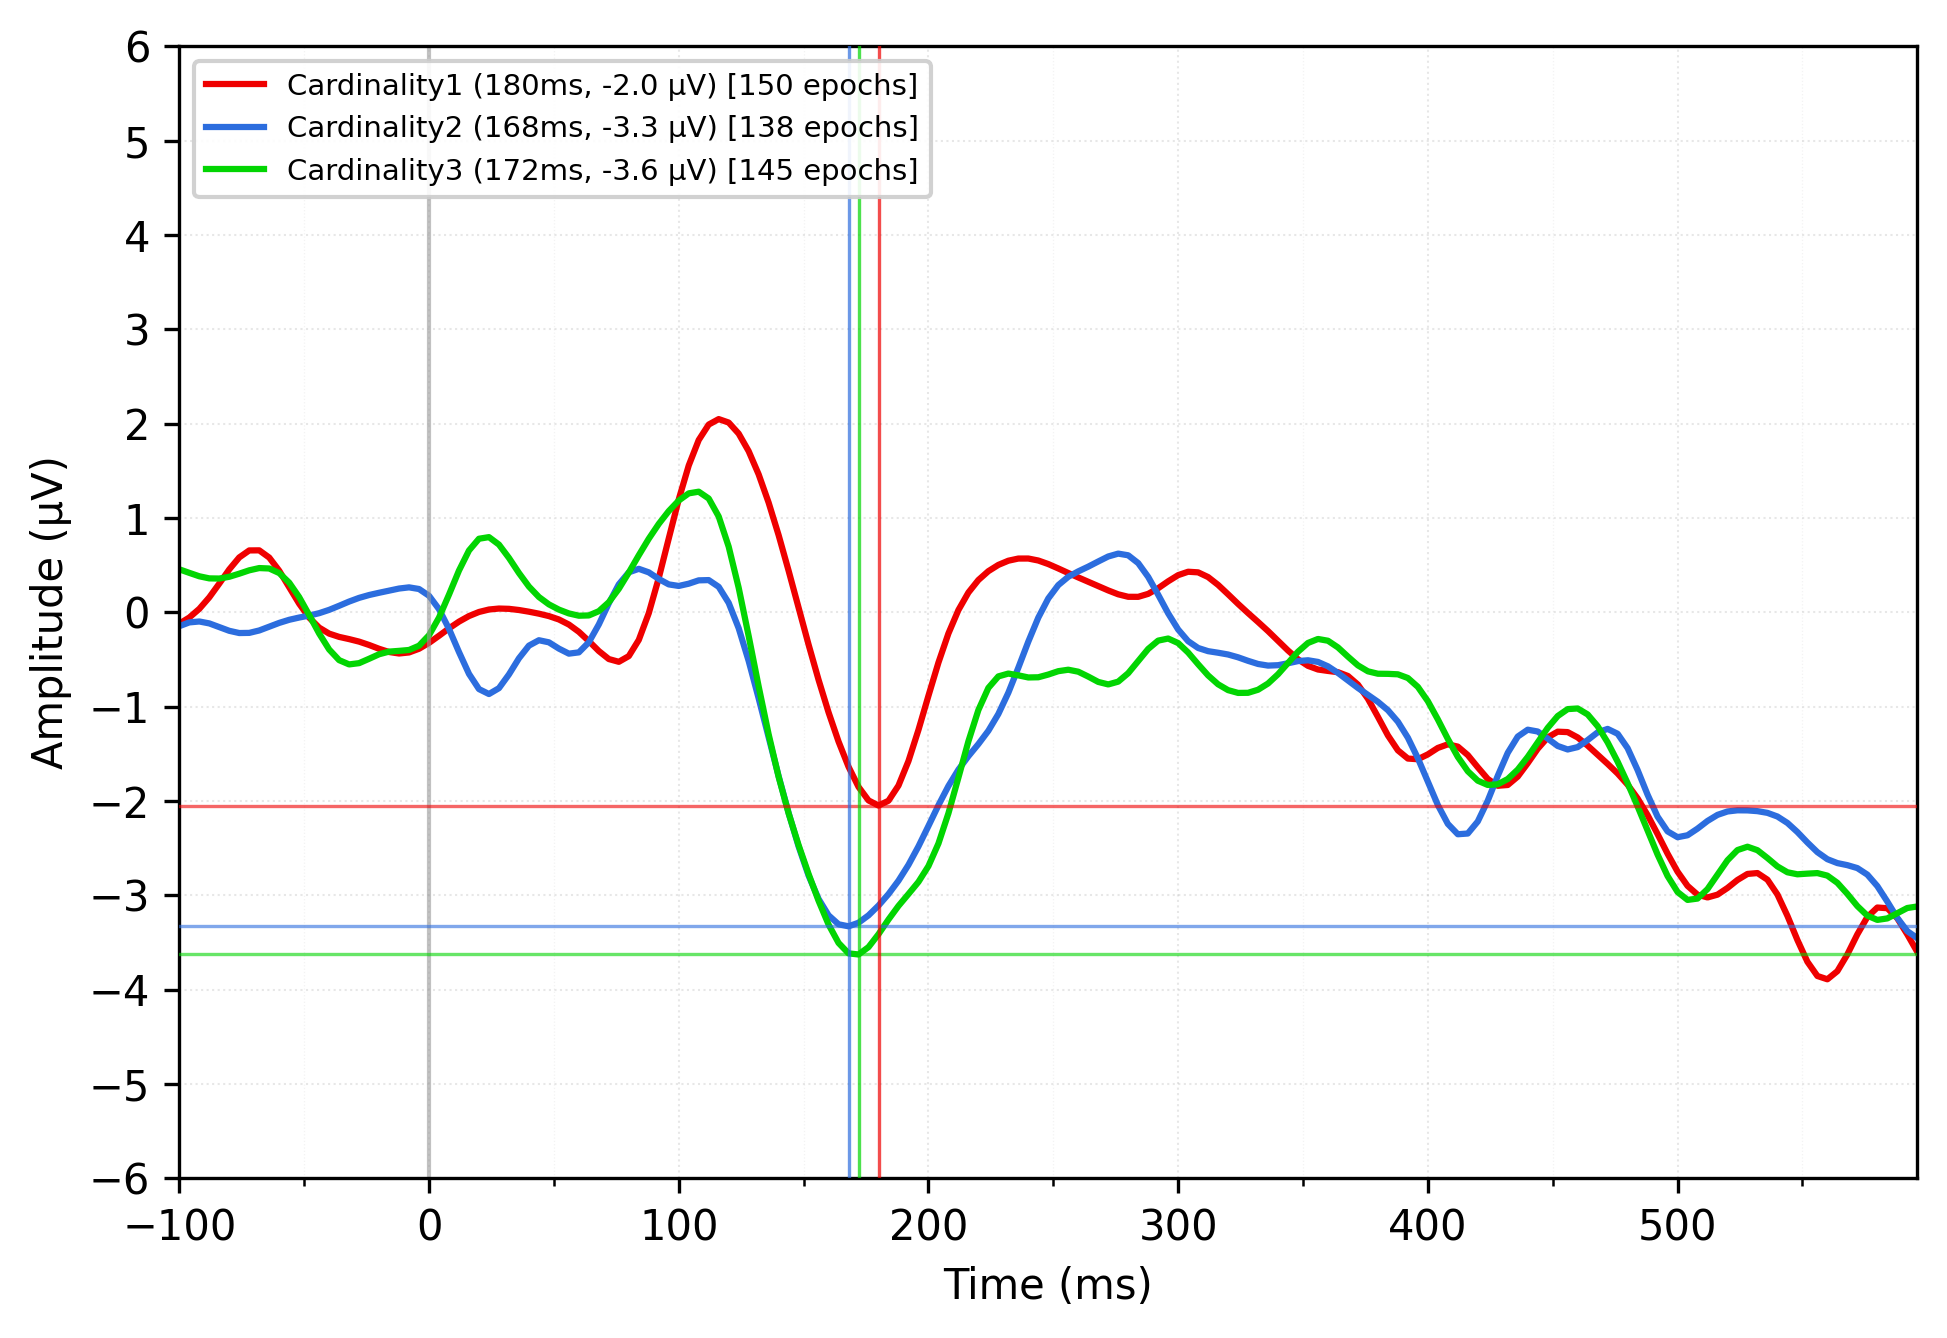
\includegraphics[width=0.43\linewidth]{../docs/assets/plots/cardinality_within_small/cardinality_within_small-N1-no_topo.png} &
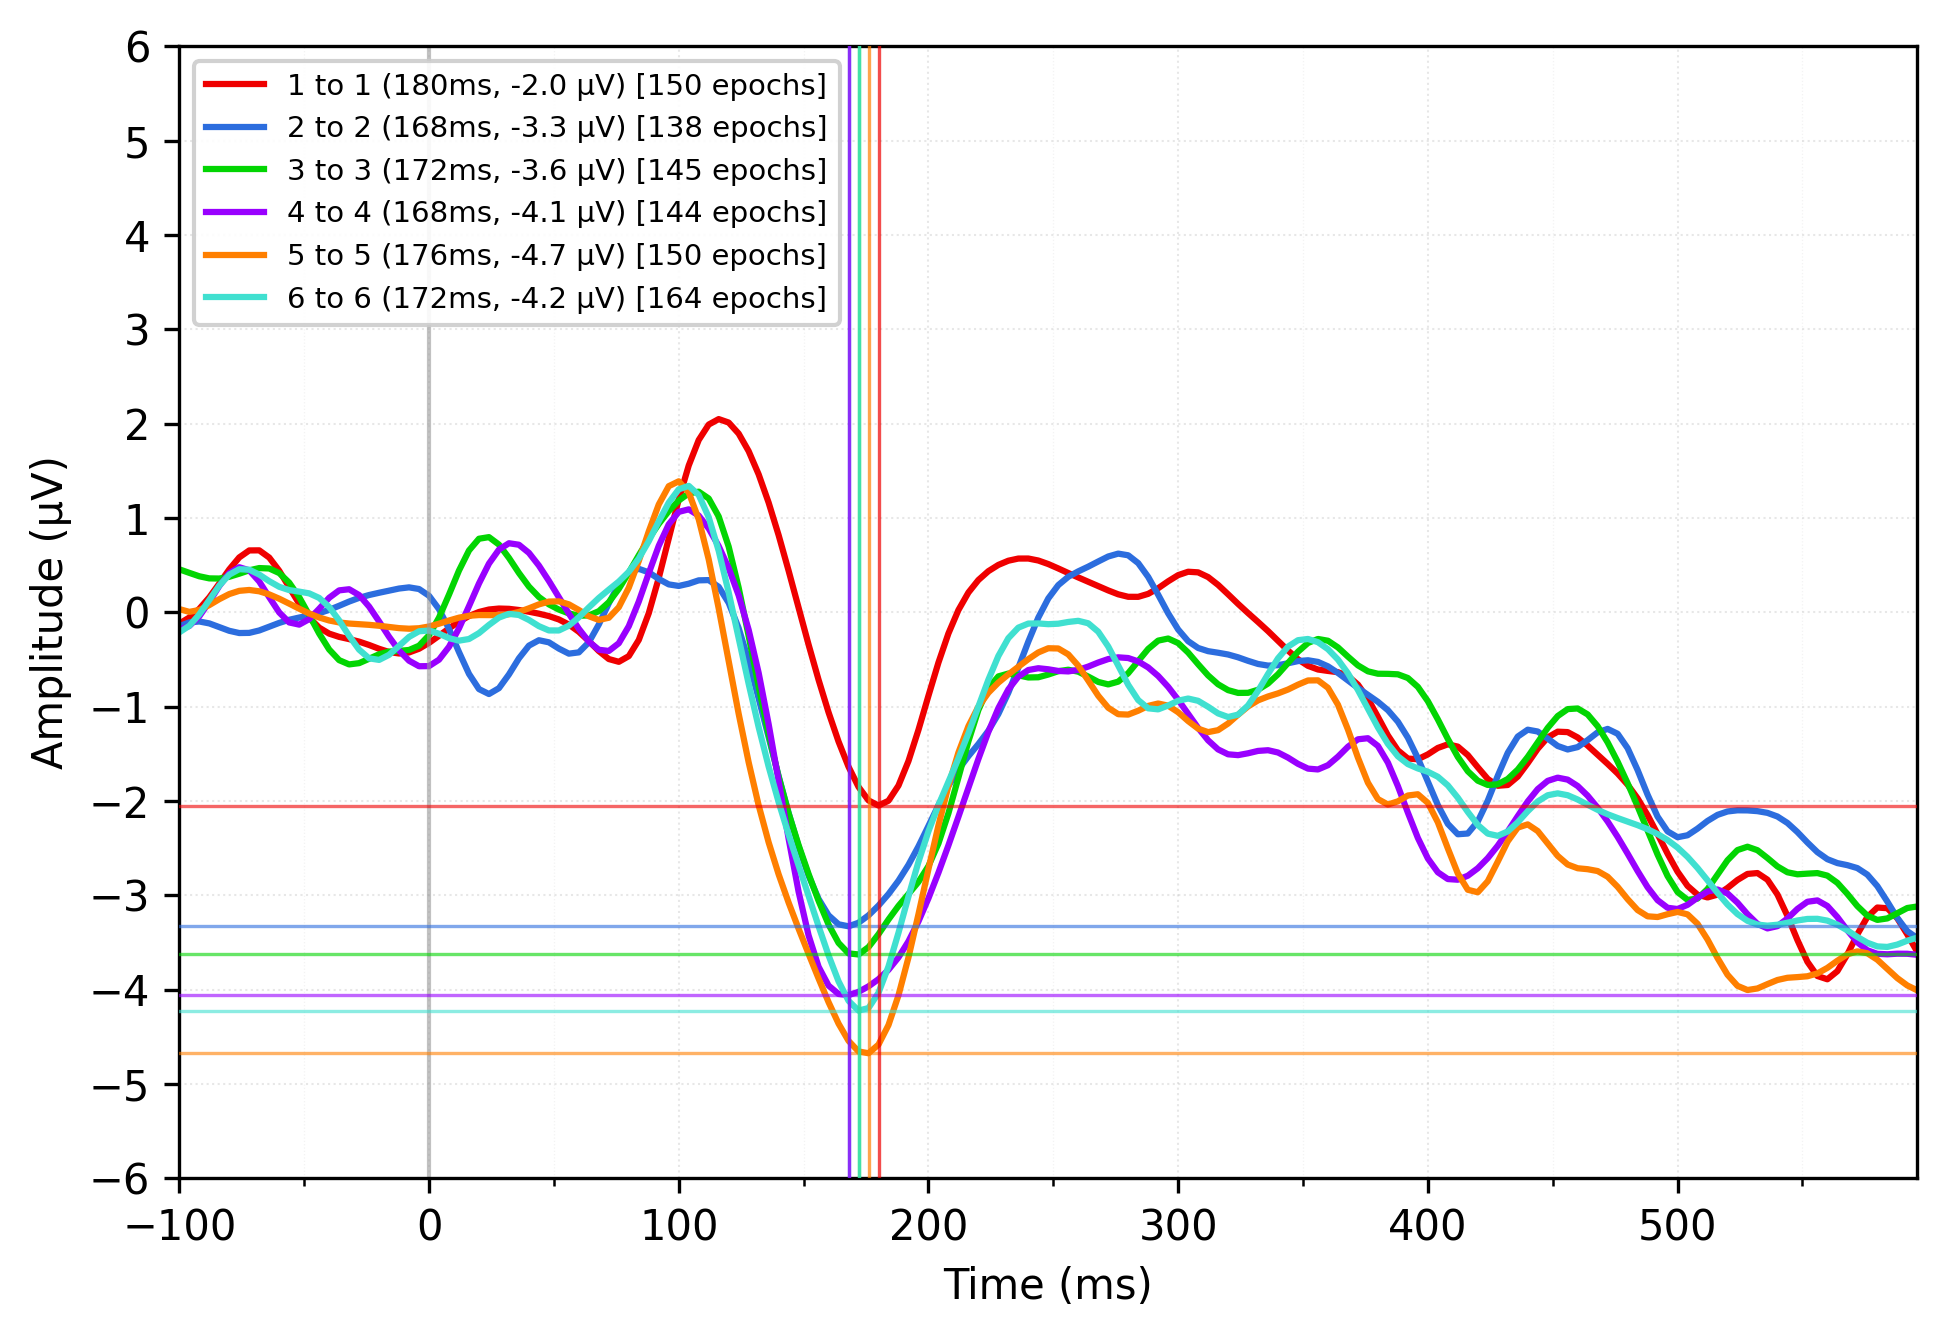
\includegraphics[width=0.43\linewidth]{../docs/assets/plots/cardinality_all/cardinality_all-N1-no_topo.png} \\
[0.12em]
{\fontsize{14}{17}\selectfont N1 within small (1-3)} &
{\fontsize{14}{17}\selectfont N1 across full cardinality} \\
\end{tabular}
\end{center}

\SmallText
\textbf{Fig. 4.} Curated ERP panel highlighting frontal change detection (MMN-like) and posterior N1 scaling.
\end{tcolorbox}

\vspace{0.12in}

\begin{tcolorbox}[posterbox]
\SectionTitle{Interpretation and Conclusion}
\SmallText
\begin{itemize}
  \item Larger numerical distance yields faster RT, and Decreasing transitions yield higher accuracy.
  \item Frontal MMN-like activity is robust during active change monitoring.
  \item Posterior N1 patterns align with small-number sensitivity and distance-dependent modulation.
  \item Together, results support interacting direction and magnitude computations.
\end{itemize}

\textbf{Contact:} vsr2116@tc.columbia.edu
\end{tcolorbox}

\vspace{0.12in}

\begin{tcolorbox}[posterbox]
\SectionTitle{References}
{\fontsize{14}{17}\selectfont
\begin{itemize}
  \item Hyde, D. C., \& Spelke, E. S. (2012). \textit{Human Brain Mapping, 33}(9), 2189-2203. doi:10.1002/hbm.21352
  \item Gordon, P. (1994, July). Innumerate Amazonians and Kronecker's Theism: One-two-many systems and the artificialism of number. European Society for Philosophy and Psychology, Paris, France.
  \item Polich, J. (2007). \textit{Clinical Neurophysiology, 118}(10), 2128-2148. doi:10.1016/j.clinph.2007.04.019
  \item Polich, J. (2011). In Kappenman \& Luck (Eds.), \textit{Oxford handbook of ERP components} (pp. 159-188). doi:10.1093/oxfordhb/9780195374148.001.0001
  \item Temple, E., \& Posner, M. I. (1998). Brain mechanisms of quantity are similar in 5-year-old children and adults. \textit{PNAS, 95}(13), 7836-7841.
\end{itemize}
}
\end{tcolorbox}
